\documentclass[a4paper,11pt,onecolumn,oneside,UTF8]{article}

\usepackage{ctex}     % 中文支持
\usepackage{amsthm,amsmath,amssymb}
\usepackage{mathrsfs}
\usepackage{bm}       % 公式中的粗体字符(用命令\boldsymbol)
\usepackage{graphicx, subfig}
\usepackage{caption}
\usepackage{float}
\usepackage{color}
\usepackage{enumerate}
\usepackage{multirow}
\usepackage{pgfplots}
\usepackage{tikz}
\usepackage{listings}
\usepackage[colorlinks,linkcolor=blue]{hyperref}

\addtolength{\topmargin}{-54pt}
\setlength{\oddsidemargin}{-0.9cm}  % 3.17cm - 1 inch
\setlength{\evensidemargin}{\oddsidemargin}
\setlength{\textwidth}{18.00cm}
\setlength{\textheight}{24.00cm}    % 24.62
\lstset{
 columns=fixed,       
 frame=none,                                          % 不显示背景边框
 backgroundcolor=\color[RGB]{245,245,244},            % 设定背景颜色
 numberstyle=\footnotesize\color{darkgray},           % 设置数字样式
 commentstyle=\it\color[RGB]{0,96,96},                % 设置代码注释的格式
 stringstyle=\rmfamily\slshape\color[RGB]{128,0,0},   % 设置字符串格式
 showstringspaces=false,                              % 不显示字符串中的空格
%  language=bash,                                       % 设置语言
%  numbers=left,                                        % 在左侧显示行号
%  numberstyle=\tiny\color{gray},                       % 设定行号格式
%  keywordstyle=\color[RGB]{40,40,255},                 % 设定关键字颜色
}

\begin{document}

\begin{center}
      \Large\textbf{Answer of Assignment 5\\分类器集成+数据聚类}
\end{center}

\begin{flushright}
      2020E8017782032\_蒲尧
\end{flushright}

\section*{第一部分:简述题}

\begin{enumerate}
      \item 请简述 adaboost 算法的设计思想和主要计算步骤。
      \item 请从混合高斯密度函数估计的角度,简述K-Means聚类算法的原理(请主要用文字描述,
            条理清晰);请给出 K-Means 聚类算法的计算步骤;请说明哪些因素会影响 K-Means 算
            法的聚类性能。
      \item 请简述谱聚类算法的原理,给出一种谱聚类算法(经典算法、Shi 算法和 Ng 算法之一)
            的计算步骤;请指出哪些因素会影响聚类的性能。
\end{enumerate}

\section*{第二部分: 计算机编程(第1题必做,第2题选做)}
\begin{enumerate}
      \item 现有 1000 个二维空间的数据点,可以采用如下 MATLAB 代码来生成:
            \begin{lstlisting}[language=MATLAB]
Sigma = [1, 0; 0, 1];
mu1 = [1, -1];
x1 = mvnrnd(mu1, Sigma, 200);
mu2 = [5.5, -4.5];
x2 = mvnrnd(mu2, Sigma, 200);
mu3 = [1, 4];
x3 = mvnrnd(mu3, Sigma, 200);
mu4 = [6, 4.5];
x4 = mvnrnd(mu4, Sigma, 200);
mu5 = [9, 0.0];
x5 = mvnrnd(mu5, Sigma, 200);
% Obtain the 1000 data points to be clustered
X = [x1; x2; x3; x4; x5];
% Show the data point
plot(x1(:,1), x1(:,2), 'r.'); hold on;
plot(x2(:,1), x2(:,2), 'b.');
plot(x3(:,1), x3(:,2), 'k.');
plot(x4(:,1), x4(:,2), 'g.');
plot(x5(:,1), x5(:,2), 'm.');
    \end{lstlisting}
            在运行完上述代码之后,可以获得 1000 个数据点,它们存储于矩阵 X 之中。X 是一个
            行数为1000列数为2的矩阵。即是说,矩阵X的每一行为一个数据点。另外,从上述MATLAB
            中可见,各真实分布的均值向量分别为 mu1, mu2, mu3, mu4, mu5。\\
            提示:在实验中,生成一个数据矩阵 X 之后,就将其固定。后续实验均用此数据集,以
            便于分析算法。\\
            请完成如下工作:
            \begin{enumerate}[(1). ]
                  \item 编写一个程序,实现经典的 K-均值聚类算法;
                  \item 令聚类个数等于 5,采用不同的初始值,报告聚类精度、以及最后获得的聚类中心,
                        并计算所获得的聚类中心与对应的真实分布的均值之间的误差。
            \end{enumerate}
      \item
            关于谱聚类。有如下 200 个数据点,它们是通过两个半月形分布生成的。如图所示:\\
            \begin{figure}[H]
                  \centering
                  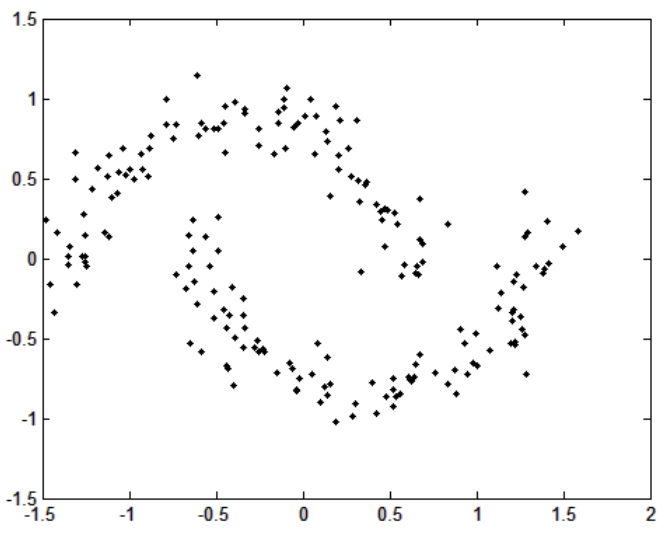
\includegraphics[width=.8\textwidth]{hw5_1.png}
                  \caption{ 本题数据点分布(具体附后) }
                  \label{img1}
            \end{figure}

            \begin{enumerate}[(1). ]
                  \item 请编写一个谱聚类算法,实现“Normalized Spectral Clustering—Algorithm 3 (Ng 算法)”。
                  \item 设点对亲和性(即边权值)采用如下计算公式:
                        $$
                              w_{ij}=exp\left(-\frac{||\bm x_i-\bm x_j||_2^2}{2\sigma^2}\right)
                        $$
                        同时,数据图采用 k-近邻方法来生成(即是说,对每个数据点 $x_i$ ,首先在所有样本
                        中找出不包含 $x_i$ 的 $k$ 个最邻近的样本点,然后 $x_i$ 与每个邻近样本点均有一条边相
                        连,从而完成图构造)。注意,为了保证亲和度矩阵 $\bm W$  是对称矩阵,可以令
                        $\bm W=(\bm W^T+\bm W)/2$, 其中,$\bm W^T$示 表示 $\bm W$ 的转置矩阵。
                        假设已知前 100 个点为一个聚类,后 100 个点为一个聚类,请分析分别取不同的 $\sigma$ 值
                        和 $k$ 值对聚类结果的影响。(本题可以给出关于聚类精度随着 $\sigma$ 值和 $k$ 值的变化曲线。
                        在实验中,可以固定一个,变化另一个)。
            \end{enumerate}

\end{enumerate}

\begin{enumerate}[附注1:]
      \item  聚类精度 Accu 计算如下:
            $$
                  Accu=\frac{n_1+n_2}{n}
            $$
            其中,$n_1$ 表示正确的属于第一个聚类的样本点的个数;$n_2$ 表示正确的属于第二个聚类
            的样本点的个数;$n$ 表示样本点的总数。
      \item 200 个样本如下 (其中,$\bm X$ 的每一行代表一个数据点):
            \href{https://github.com/Allenem/PatternRecognition/blob/main/hw5/data_hw5.txt}{data文件}
\end{enumerate}


\section*{第一部分回答}

\begin{enumerate}
      \item
            \begin{enumerate}[(1)]
                  \item
                        Adaboost算法的\textbf{设计思想}就是训练一系列弱分类器,然后组合成一个强分类器。具体有两方面的内容要做:\\
                        1)如何改变训练数据的权重?提高前一轮弱分类器错分样本的权重,降低正确分类样本的权重;\\
                        2)如何调整弱分类器的权重?采用加权多数表决的方法。即加大分类错误率较低的分类器的权重,减小错误率高的分类器权重。\\
                  \item
                        \textbf{主要计算步骤:}\\
                        1)初始化训练数据权值分布:$D_1=\left\{w_{11},w_{12},...,w_{1n}\right\}, w_1i=1/n, i=1,2,...,n$\\
                        2)对于m=1,2,...,M\\
                        2a)学习具有权值分布$D_m$的训练数据,学习基本分类器:$G_m\left(\bm X\right): \bm X → \left\{-1,+1\right\}$\\
                        2b)计算$G_m\left(\bm X\right)$在训练数据集上的分类加权错误率:$e_m=\sum\limits_{i=1}^nw_{mi}\underbrace{I(G_m\left(\bm X_i\neq y_i\right))}_{truth\quad function}$\\
                        2c)计算$G_m\left(\bm X\right)$的贡献系数,即第m个分类器的权值:$\alpha_m=1/2\ln \frac{1-e_m}{e_m}$,$e_m$越大,权重$\alpha_m$越小\\
                        2d)更新训练数据集的权重分布:$D_{m+1}=\left\{w_{m+1,1},w_{m+1,2},...,w_{m+1,n}\right\}$\\
                        $$
                              \begin{aligned}
                                    w_{m+1,i}       & =\frac{w_{mi}}{Z_m}×exp\left(-\alpha y_iG_m\left(X_i\right)\right)       \\
                                    Where \quad Z_m & =\sum\limits_{i=1}^nw_{mi}exp\left(-\alpha y_iG_m\left(X_i\right)\right)
                              \end{aligned}
                        $$
                        3)构造基本分类器的线性组合:$f\left(\bm X\right)=\sum\limits_{m=1}^M\alpha_mG_m\left(\bm X\right)$。\\
                        对于二分类器:$G\left(\bm X\right)=sign\left(f\left(\bm X\right)\right)=sign\left(\sum\limits_{m=1}^M\alpha_mG_m\left(\bm X\right)\right)$。
            \end{enumerate}
      \item
            \begin{enumerate}[(1)]
                  \item K-Means聚类算法的\textbf{原理}\\
                        假设每个样本以概率为1属于某个类,则\\
                        $$
                              \begin{aligned}
                                    P\left(\omega_i|x_k,\hat{\mu}\right) & =\left\{\begin{array}{ll}
                                          1, & x_k \in \omega_i;   \\
                                          0, & x_k \notin \omega_i
                                    \end{array}
                                    \right.                                                                                                                                  \\
                                    \hat{P}\left(\omega_i\right)         & = n_i/n                                                                                           \\
                                    \hat{\mu}_i                          & =\frac{1}{n_i}\sum\limits_{k=1}^{n_i}x_k^i                                                        \\
                                    \hat{\Sigma}_i                       & =\frac{1}{n_i}\sum\limits_{k=1}^{n_i}\left(x_k^i-\hat{mu}_i\right)\left(x_k^i-\hat{mu}_i\right)^T
                              \end{aligned}
                        $$
                        K-Means聚类算法是一种基于距离的聚类算法,即先随机给出类中心,通过不断计算距离归类和重新计算类中心的迭代最终确定趋于正确的类中心。
                  \item K-Means聚类算法的计算步骤\\
                        先引入两个假设:\\
                        1)各类出现的先验概率均相等\\
                        2)每个样本以概率1属于某个类(即后验概率0-1近似)\\
                        \textbf{步骤:}\\
                        1)根据给定的K值划分,可以随机选择K个点作为类中心;\\
                        2)计算每个点到各个类中心的距离,将该点归到距离最近的类中心的Cluster类下;\\
                        3)重新计算每个Cluster的类中心;\\
                        4)重复2和3,直到类中心在某个精度范围不变化或者到达最大迭代次数。
                  \item \textbf{影响因素}\\
                        – 必须事先给定簇的个数,且对初始值敏感;\\
                        – 不适合于发现非凸曲面的簇以及大小相差很大的簇;\\
                        – 对噪声、孤立数据点、野点很敏感。
            \end{enumerate}
      \item
            \begin{enumerate}[(1)]
                  \item 谱聚类算法的\textbf{原理}\\
                        – 从图切割的角度,聚类就是要找到一种合理的分割图的方法, 分割后能形成若干个子图。
                        连接不同子图的边的权重尽可能小,子图内部边权重尽可能大。\\
                        – 谱聚类算法建立在 图论中的谱图理论基础之上,其本质是将聚类问题转化为一个
                        图上的关于顶点划分的最优问题。\\
                        – 谱聚类算法建立在 点对亲和性基础之上,理论上能对任意分布形状的样本空间进行聚类。\\
                        – 算法的核心是将原始的数据点 $x_i$ 转换为在特征空间的数据点 $y_i$ ,在新的空间对原始数据进行描述
                  \item 谱聚类算法的\textbf{计算步骤}\\
                        – 利用点对之间的相似性,构建亲和度矩阵$\mathbb{W}$;\\
                        – 构建拉普拉斯矩阵:\\
                        \quad • Classical: $\mathbb{L} = \mathbb{D}-\mathbb{W}$\\
                        \quad • Shi's Algorithm: $\mathbb{L}_{rw} = \mathbb{D}^{-1}\mathbb{L}$\\
                        \quad • Ng's Algorithm: $\mathbb{L}_{sym} = \mathbb{D}^{-1/2}\mathbb{L}\mathbb{D}^{-1/2}$\\
                        – 求解拉普拉斯矩阵最小的k个特征值{$\lambda_1,\lambda_2,...,\lambda_k$}对应的特征向量{$\vec{u}_1,\vec{u}_2,...,\vec{u}_k$}(通常舍弃零特征所对应的分量全相等的特征向量);\\
                        \quad • Classical: $\mathbb{L}\vec{u} =  \lambda \vec{u}$\\
                        \quad • Shi's Algorithm: $\mathbb{L}_{rw}\vec{u} =  \lambda \mathbb{D}\vec{u}$\\
                        \quad • Ng's Algorithm: $\mathbb{L}_{sym}\vec{u} =  \lambda \vec{u}$\\
                        – 由这些特征向量构成样本点的新特征(Ng的特征向量需要归一化),大小n×k,采用K-means等聚类方法完成最后的聚类。
                  \item \textbf{影响因素}\\
                        相似度的计算方法,拉普拉斯矩阵、特征向量的归一化方法,局部链接数目,聚类数目和方法,等等。
            \end{enumerate}
\end{enumerate}

\section*{第二部分回答}

\begin{enumerate}
      \item

            代码见如下文件:
            \href{https://github.com/Allenem/PatternRecognition/blob/main/hw5/PR_hw5_1.m}{MATLAB文件1主程序},
            \href{https://github.com/Allenem/PatternRecognition/blob/main/hw5/K_Means.m}{MATLAB文件2KMeans函数},
            \href{https://github.com/Allenem/PatternRecognition/blob/main/hw5/hw_5_kmeans.py}{Kmeans的Python实现}。
            效果图如下,十字是最初算得的类中心,颜色与类别有差异;圆圈是重排序之后的类中心,颜色与类别无差异。
            由实验结果可知,初始化的均值会影响最终的类中心收敛,下面的第一幅图显然收敛到了两类的中间,而第二幅图由于初始的均值设置合理聚类准确度较高。
            说明一定的先验知识对聚类很有帮助:\\
            \begin{figure}[H]
                  \centering
                  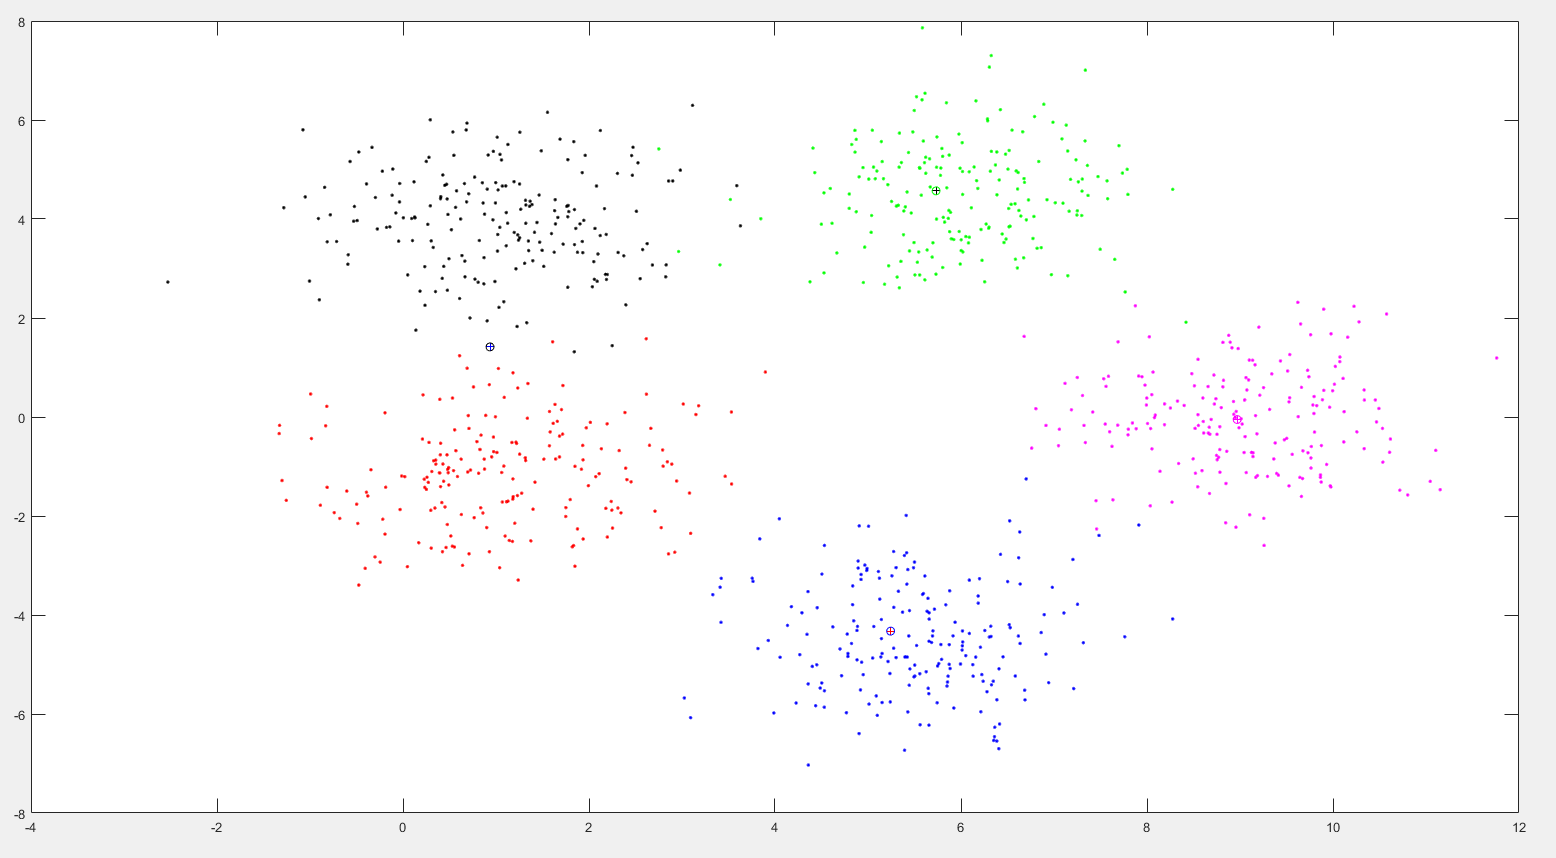
\includegraphics[width=.8\textwidth]{hw5_2.png}
                  \caption{ 聚类准确率77.8\%,均方误差1.1389图像 }
                  \label{img2}
            \end{figure}
            \begin{figure}[H]
                  \centering
                  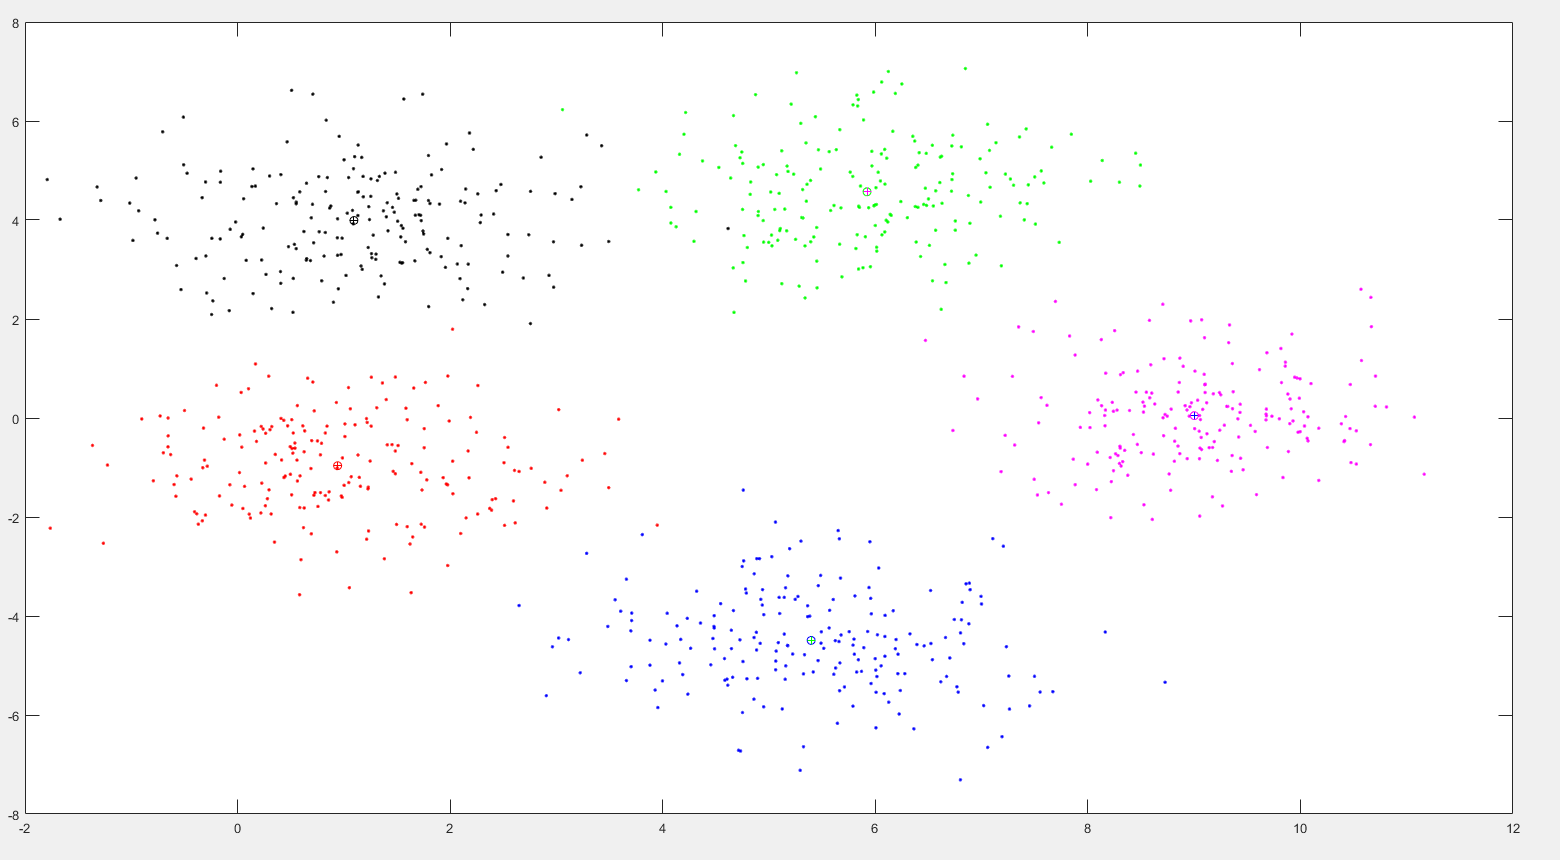
\includegraphics[width=.8\textwidth]{hw5_3.png}
                  \caption{ 聚类准确率99.5\%,均方误差0.0121图像 }
                  \label{img3}
            \end{figure}

      \item
            代码见如下文件:
            \href{https://github.com/Allenem/PatternRecognition/blob/main/hw5/hw5_spectral_cluster.py}{Ng算法谱聚类的Python实现}。
            效果图,准确度随着$\sigma$和$k$变化的曲线如下:\\
            \begin{figure}[H]
                  \centering
                  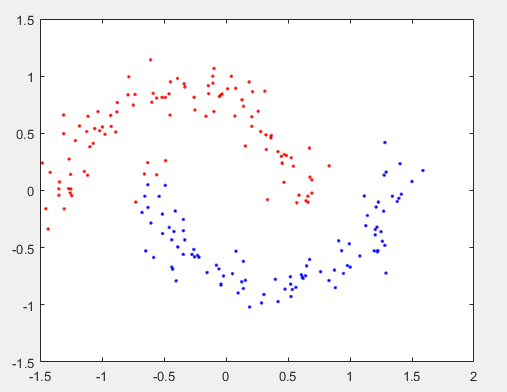
\includegraphics[width=.8\textwidth]{hw5_4.png}
                  \caption{ Ng算法谱分类效果图 }
                  \label{img4}
            \end{figure}
\end{enumerate}

\end{document}